%%%%%%%%%%%%%%%%%%%%%%%%%%%%%%%%%%%%%%%%%%%%%%%%%%%
%
%  New template code for TAMU Theses and Dissertations starting Fall 2012.  
%  For more info about this template or the 
%  TAMU LaTeX User's Group, see http://www.howdy.me/.
%
%  Author: Wendy Lynn Turner 
%	 Version 1.0 
%  Last updated 8/5/2012
%
%%%%%%%%%%%%%%%%%%%%%%%%%%%%%%%%%%%%%%%%%%%%%%%%%%%

%%%%%%%%%%%%%%%%%%%%%%%%%%%%%%%%%%%%%%%%%%%%%%%%%%%%%%%%%%%%%%%%%%%%%%%
%%%                           SECTION I
%%%%%%%%%%%%%%%%%%%%%%%%%%%%%%%%%%%%%%%%%%%%%%%%%%%%%%%%%%%%%%%%%%%%%%

\renewcommand*{\thefootnote}{\fnsymbol{footnote}}
\chapter[\uppercase{Targeted Observations with the VIRUS Prototype Instrument}]{\uppercase{Targeted Observations with the VIRUS Prototype Instrument}\symbolfootnote[1]{Reprinted with permission from ``Introduction: The Importance of Research'' by AUTHOR et al., 2015. The Astrophysical Journal, Volume XYZ, Issue X, article id. XY, XY pp., Copyright 20XX by the American Astronomical Society.} }
\renewcommand*{\thefootnote}{\arabic{footnote}}
\setcounter{footnote}{0}

\section{Introduction} 
Many large area-sky surveys both currently underway and upcoming are prioritizing the identification of clusters for both detailed studies of cosmology and for fundamental physical studies of the individual clusters. At present, the greatest number of clusters are being confirmed using large millimeter wave surveys with the South Pole Telescope (SPT; \citealt{Carlstrom2011}) or the Atacama Cosmology Telescope (ACT; \citealt{Swetz2011}). These observations rely on the Sunyaev-Zel'dovich effect (SZE; \citealt{Sunyaev1972}) which uses the up-scattering of cosmic microwave background (CMB) photons to both identify the cluster and to estimate its mass. However, deep, wide field optical surveys, such as the Dark Energy Survey (DES; \citealt{DES2005}) and planned Large Synoptic Survey Telescope (LSST; \citealt{LSST2012}) will discover many more clusters at increasing lower mass in the near future. Such surveys will employ the richness of the individual clusters as a cluster mass proxy, and as such, will rely on followup observations to better constrain the absolute scale and the scatter in the richness-mass relation. But, as the number of clusters grows to many tens of thousands, individual followup becomes unfeasible. Therefore, we rely on well calibrated observable-mass relationships to estimate the masses of the observed clusters.

Unfortunately, mass is not directly observable, so we must estimate it through another discernible cluster property. Observed X-ray temperatures and luminosities correlate tightly with a cluster's dynamical mass \citeeg{Mantz2010, Rykoff2014}, especially for dynamically relaxed clusters \citeeg{Mantz2015}. Observations of the SZE can provide accurate estimations of mass \citeeg{Vanderlinde2010, Sehgal2011}, but can be effected by the physics of the intracluster medium \citeeg{Pipino2010} and the ability to detect low mass galaxy clusters is currently limited by technology \citeeg{Carlstrom2002a}. The richness \citeeg{Abell1958,Rykoff2012}, the weighted number of cluster member galaxies within a scale aperture, is a promising method which has been shown to correlate strongly with cluster mass \citeeg{Rozo2010}. 

The richness is already being used in many optical studies \citeeg{Ruel2014, Sifon2015}, but the absolute mass scale and more importantly the  intrinsic scatter in the relation are currently under active investigation \citeeg{Rozo2015, Saro2015, Baxter2016, Farahi2016, Simet2016}. These systematics remain the major source of uncertainty in deriving cosmological constraints from cluster abundances and testing structure growth in a $\Lambda$CDM universe. To realize fully the promise of the large samples from DES and LSST, we must measure both the absolute mass scale and scatter in the optical-richness mass estimator using independent methods.

The Hobby Eberly Dark Energy Experiment (HETDEX; \citealt{Hill2008}) is a forthcoming blind spectroscopic survey that offers the ability to calibrate accurately the optical richness-mass relation for a significant number of galaxy clusters at both extremes of the mass scale. At present, because HETDEX is designed to measure the dark energy equation of state at $z\sim2$, and the applicability to galaxy cluster science has not yet been investigated.  We began this investigation with \defcitealias{Boada2016}{Paper I}\cite{Boada2016} (hereafter \citetalias{Boada2016}). We find the blind spectroscopic observations of HETDEX are capable of accurately estimating galaxy cluster masses over the range of redshifts and cluster masses covered by the study. We find that using a machine learning approach where several cluster observables are combined, we estimate cluster masses to a similar level of precision as a fully targeted survey. The ability of HETDEX to further constrain optically derived masses is of paramount importance to upcoming large photometric surveys. This study provides insight into how well a HETDEX type survey will constrain mass estimations and cosmological parameters in the future.

In this work, we present a pilot study of ten massive galaxy clusters using integral field spectroscopy with the Mitchell Spectrograph as a pilot program for HETDEX. The second installment of this two part work, the goal of this study is to obtain spectroscopic redshifts of the individual cluster galaxies, determine the velocity dispersion and to infer each cluster's dynamical mass. This allows us to compare the inferred mass with other mass estimators (\eg, the clusters in this sample have deep \textit{Chandra} or \textit{XMM-Newton} X-ray data, and richness measurements) with the aim of better characterizing the scatter in the richness-mass relation, $\sigma_{M|\lambda}$.

The layout of this work is the following. In Section~\ref{2sec:design} we discuss the target selection and the setup of the Mitchell Spectrograph used to conduct the observations. Section~\ref{2sec:data reduction} describes the methods and tools used to reduce the observations. We present our redshift catalog, cluster members and cluster dynamical properties in Section~\ref{2sec:analysis}. We discuss a machine learning based alternative to a traditional power law estimate of cluster mass in Section~\ref{2sec:ML methods} In Section~\ref{2sec:results}, we compare and discuss the different mass estimations and remark on the applicability of these methods for the study of the optical richness-cluster mass relationship.  Finally, we summarize this work in Section~\ref{2sec:summary}.

Throughout this paper, we adopt the following cosmological model from the Buzzard simulations (see Section~\ref{2sec:ML methods}): $\Omega_\Lambda = 0.714$, $\Omega_M = 0.286$, and $H_0= 70$ \kms \mpc, assume a Chabrier initial mass function (IMF; \citealt{Chabrier2003}), and use AB magnitudes \citep{Oke1974}.

\section{Design}\label{2sec:design} 
\subsection{Target Selection}\label{2sec:selection} 

\begin{landscape}
	\begin{table}
	\caption[Basic properties of the ten galaxy clusters targeted with the MS.]{Basic properties of the ten galaxy clusters targeted with the MS: Column 1: Our internal cluster name; Column 2: An alternative cluster name; Column 3: The right ascension of the cluster; Column 4: The declination of the cluster; Column 5: the nominal (often photometric) cluster redshift; Column 6: The date of our observations.} 
	\begin{tabular}{lccccc} 
		\hline 
		Cluster & Alt. Name & RA (J2000) & DEC (J2000) & $z$ & Obs. Date\\
		(1) & (2) & (3) & (4) & (5) & (6) \\
		\hline \hline
		VCSJ010455.4+000336.3 & SOGRAS J0104+0003 & 01:04:55.369 & +00:03:36.28 & 0.277 & August, 2012 \\
		VCSJ133520.1+410004.1 & Abell 1763 & 13:35:20.092 & +41:00:04.12 & 0.223 & May, 2012 \\
		VCSJ140102.0+025242.6 & Abell 1835 & 14:01:01.965 & +02:52:42.63 & 0.252 & May, 2012 \\
		VCSJ153656.3+242431.6 & MaxBCG J234.23439+24.40877 & 15:36:56.253 & +24:24:31.60 & 0.226 & May, 2012 \\ 
		VCSJ164019.8+464241.5 & Abell 2219 & 16:40:19.812 & +46:42:41.51 & 0.225 & May, 2012 \\
		VCSJ172227.2+320757.2 & Abell 2261 & 17:22:27.182 & +32:07:57.24 & 0.224 & May, 2012 \\
		VCSJ211849.1+003337.3 & MaxBCG J319.70446+00.56035 & 21:18:49.069 & +00:33:37.33 & 0.270 & August, 2012 \\
		VCSJ215422.9+003723.5 & Abell 2392 & 21:54:22.936 & +00:37:23.48 & 0.223 & August, 2012\\
		XMMXCSJ124425.9+164758.0 & WHL J124425.4+164756 & 12:44:25.203 & +16:47:48.00 & 0.235 & May, 2013 \\
		XMMXCSJ125650.2+254803.2 & \nd & 12:56:49.999 & +25:48:02.99 & 0.280 & May, 2013 \\
		\hline 
		\end{tabular}
		\label{2tbl:targets} 
	\end{table}
\end{landscape}

We select clusters at $z=0.2-0.3$ using two different methods and for two different purposes. We optically select eight of the ten clusters from \cite{Rykoff2012} using the \textit{Sloan Digital Sky Survey} (SDSS; \citealt{Blanton2001a}) Data Release 8. These clusters have high ($\lambda>70$) observed richnesses which corresponds to $M > 2.2\times10^{14}$ \Msol, and are a combination of relaxed and unrelaxed systems. The last two clusters are selected from the \textit{XMM Cluster Survey} (XCS; \citealt{Mehrtens2012}) and correspond to individually measured X-ray temperatures of $T_X < 2.5$ keV. Such X-ray temperatures have inferred masses of $10^{14}\msol > M_{DM} > 5\times10^{13}\Msol$.

The optically selected clusters have many more members (see Table~\ref{2tbl: derived parameters}) than the X-ray selected clusters which allows us to investigate the accuracy of our mass recovery methods at both cluster and group scales. See Table~\ref{2tbl:targets} for individual cluster sky positions and associated parameters. 

\subsection{Observations} 
We use the Mitchell Spectrograph (MS; formerly known as VIRUS-P; \citealt{Hill2008a}) an integral field unit (IFU) in a square array of 246 $4\farcs24$ diameter optical fibers. This provides a $1\farcm7~\times~1\farcm7$ field-of-view (FOV) with a 1/3 filling factor. A Fairchild Instruments, 2k$\times$2k charge couple device (CCD) images the spectra from each of the 246 fibers. The spectra have approximately a gaussian profile with a 5 pixel full width at half maximum (FWHM), and each are separated by 8 pixels to minimize the amount of cross-talk between the fibers. 

There are two spectral configurations available on MS, a blue setup, 3600-5800 \AA\ and a red setup, 4600-6800 \AA. In addition, there are four volume phase holographic gratings available to disperse the light. For the purpose of this work, the lowest resolution, $\sim5$\AA, grating is used. Using $1\times1$ binning, this translates into a spectral dispersion of $\sim1.11$ \AA\ pixel$^{-1}$. 

\begin{figure}[t]
	\begin{center}
		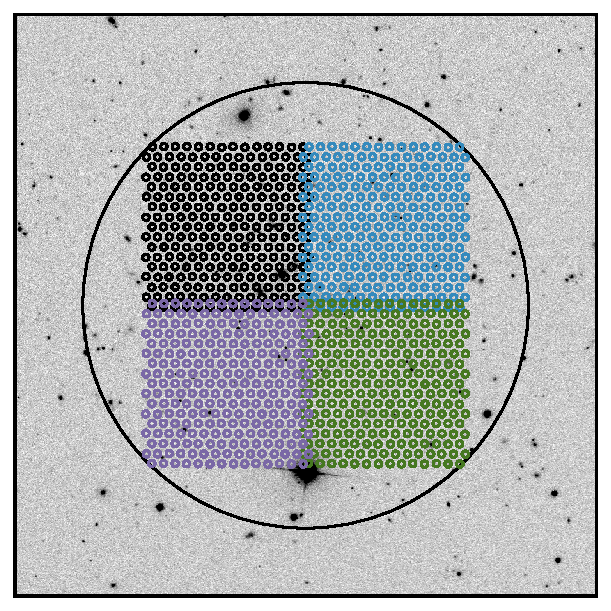
\includegraphics[width=0.6\textwidth]{./figures2/pointing.pdf} 
	\end{center}
	\caption[Basic properties of the ten galaxy clusters targeted with the MS.]{SDSS r-band image of an optically selected galaxy cluster Abell 2631 ($z=0.273$) selected from the SDSS DR8 data, and centered on the BCG. The large black circle shows the region $R<0.5$ Mpc ($r<2\farcm3$). The northeast (NE), northwest (NW), southwest (SW), and southeast (SE) fields with the fiber positions are shown in black, blue, green and purple respectively, illustrating how we survey each cluster. Nearly all galaxies within this region are associated with the cluster.}
	\label{2fig:tiles} 
\end{figure}

We use MS to target the galaxy clusters using the 5 \AAA\ grating covering a wavelength range of $4400 - 6600$ \AAA. With this instrumental setup and for galaxies $z = 0.2-0.3$, we will cover the Ca H\&K, Fe I ($\lambda 4383$), H-$\delta$, H-$\gamma$ and H-$\beta$ absorption features. Additionally, we cover emission of the \hbox{[\ion{O}{ii}]} ($\lambda\lambda 3727,3729$) doublet, H-$\beta$, and \hbox{[\ion{O}{iii}]} ($\lambda\lambda 4960,5008$), which allows for the identification of actively star-forming galaxies.

The FOV of the MS corresponds to an approximately 0.4 Mpc square region at $z = 0.2-0.3$. To ensure adequate coverage of the cluster out to a radius of 0.5 Mpc, we use four MS pointings per cluster. Figure~\ref{2fig:tiles} shows an example of the pointing pattern done on each cluster. The entire field is centered on the brightest cluster galaxy (BCG) and the individual tiles are shifted away. Furthermore, each of the four tiles are dithered at relative positions $(\Delta \alpha, \Delta \delta)=(0\farcs0,0\farcs0)$, $(-3\farcs6,-2\farcs0)$, and $(0\farcs0, -4\farcs0)$ from the origin to ensure full coverage of the FOV. Therefore, there are 736 individual spectra for each of the four fields or 2952 measurements for the cluster as a whole.

We have set exposure times to achieve spectra with signal-to-noise ratios (SNRs) $\sim3$ per spectral element (averaged over 4.6 pixels) in the continuum for objects with \sdssg\ $= 21.3$ mag (which corresponds to approximately 0.2L$^\star$ for cluster galaxies at $z = 0.2$) in 3600 seconds per pointing.. We base the expected SNR on the experience of \cite{Shetrone2010}, who achieves SNR $= 100$ per pixel in the continuum for point sources with B $=16.5$ mag at 4000 \AAA\ in 4800 seconds. We require 4 pointings to cover the full area for each cluster. Therefore, we require 1 hr/pointing $\times$ 4 pointings $= 4$ hrs on sky per cluster. Even though the field is dense with galaxies, there is sufficient ``blank'' area to allow for enough ``sky'' fibers for background subtraction.

\section{Data Reduction}\label{2sec:data reduction} 
All data are reduced using \textsc{p3d}\footnote{http://p3d.sourceforge.net/} \citep{Sandin2010} a general-use IFU reduction pipeline. The first step is to min/max-filtered average combine a minimum of 20 bias images from each night into a master-bias image, which is subtracted from each other image from the same night. Secondly, a trace mask is created from flat-fielding on the dusk or dawn sky. The fibers are fairly densely packed, so to determine the position of each spectrum in the dispersion direction each spectrum is extracted using a multi-profile deconvolution approach \citep{Sharp2010} to account for cross talk between fibers. Third, a dispersion mask for the wavelength calibration from images of Hg+Cd (for the May, 2012 observations) or Cd+Ne (for all other observations) arc lamps. The residuals between the derived wavelength solution and the known wavelengths of the emission lines is calculated from a fifth order polynomial and lie between $0.02 - 0.06$ \AAA. Finally, a fiber flat is created from the sky flats by a min/max-filtered average combine as in step one. 

We extracted the science spectra using several steps. First, we subtract the bias frames from each science frame. Next, we use \textsc{PyCosmic} \citep{Husemann2012}, integrated into \textsc{p3d} with the default parameters, to clean cosmic ray hits. Third, we use the previously created dispersion mask to wavelength calibrate the extracted spectra. Aligning the dispersion mask to bright telluric lines (namely \hbox{[\ion{O}{i}]} at 5577 \AAA) accounts for any flexure in the instrument between the images of the arc lamps and science frames. Finally, we normalize the extracted spectra using the transmission in the fiber flats from above. 

The result of this process is row-stacked spectra and associated pipeline-propagated uncertainties, where each of the 246 fibers are stored individually. A table of fiber positions maps each spectrum onto the image plane. However, for many of our observations a precise astrometric solution for the fiber positions is unknown. The position of the individual fibers can be recomputed by observing dense star fields after each telescope service in which the MS is involved. To correct our fiber positions we first identify fibers which observe stars and identify which fibers the astrometric solution indicates should contain stars. In many cases the stars are located between fibers. To account for this we use a simple Gaussian centroid weighted by the observed flux $5000 \leq \lambda \leq 5010$ \AAA\ to find the correct sky position of the star. We then shift the fiber grid to match the sky position of the stars as reported by the SDSS. Typical shifts are $0.5'' - 4''$, less than the width of a single fiber. For each observation we use as many stars as possible and combine the shifts to generate a mean offset. This offset is applied to all dithers of each observation. There is little need to obtain highly accurate fiber positions as the $4\farcs24$ fibers insures that reasonably correct positions will identify which fibers should and should not contain galaxies.

We use a simple sky subtraction scheme to remove the majority of sky contamination. Because the majority of fibers for any single pointing are empty, we use a $3\sigma$ clipped median selection to identify sky fibers and a simple mean to combine them. The result is then subtracted from every fiber. This adequately removes the bulk of sky emission lines, but often fails to completely remove the \hbox{[\ion{O}{i}]} line at 5577~\AAA. This line is masked throughout the determination of redshifts.

\begin{figure}[t]
\subfloat{%
  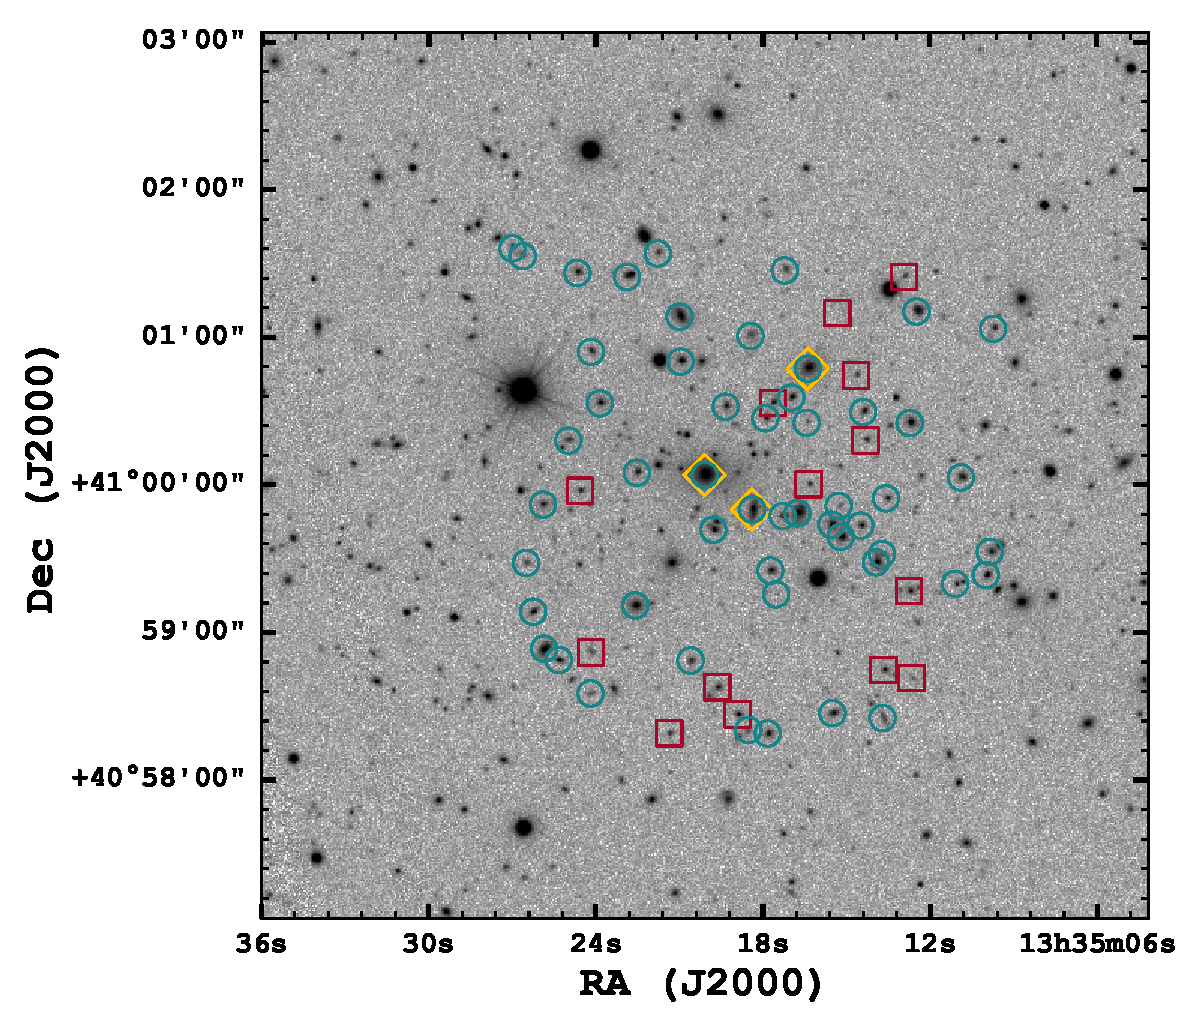
\includegraphics[width=0.5\textwidth]{./figures2/c203p83+41p0_mosaic.pdf}
}
\hfill
\subfloat{%
  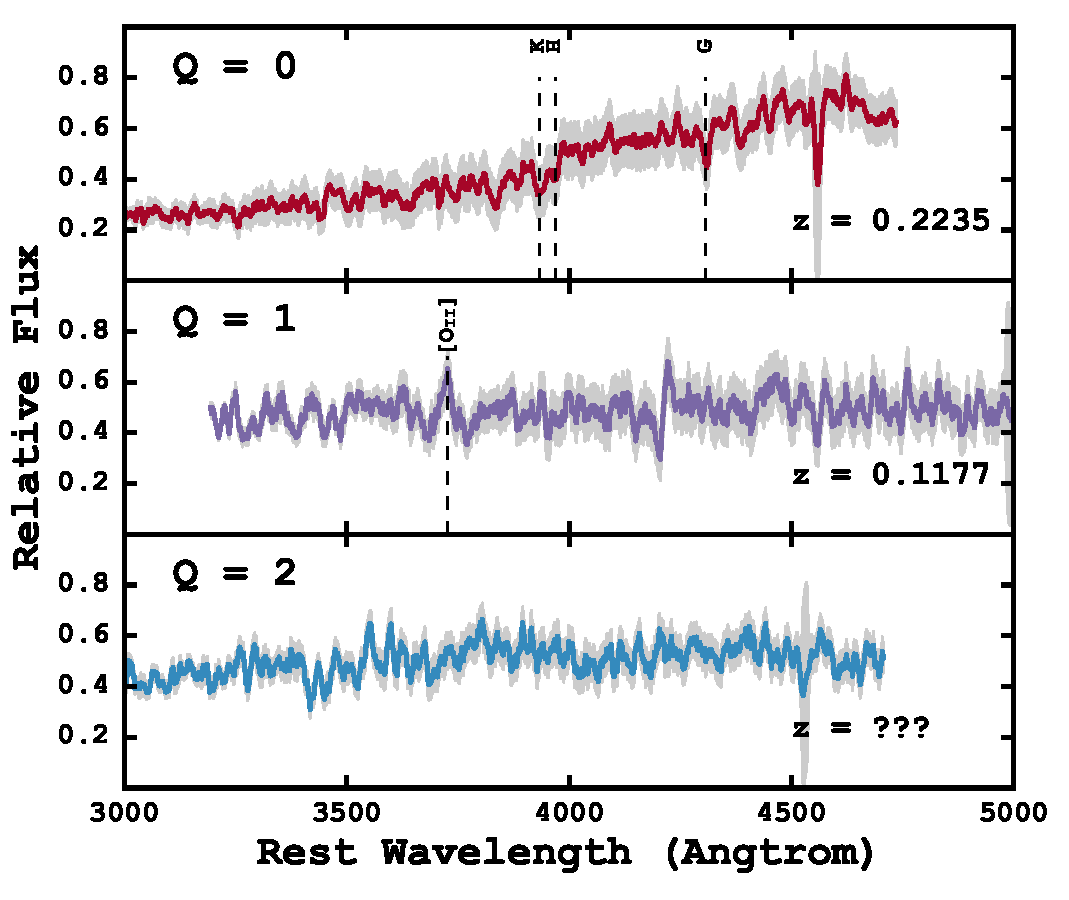
\includegraphics[width=0.5\textwidth]{./figures2/spectrum.pdf}
}
    \caption[SDSS \sdssr\ image of cluster VCSJ133520.1+410004.1 and spectra quality examples]{SDSS \sdssr\ image of cluster VCSJ133520.1+410004.1. The symbols show the position of observed galaxies. Turquoise circles indicate galaxies with $Q=0$ or $Q=1$ spectroscopic redshifts, red squares indicate galaxies where a redshift could not be reliably determined, and the yellow diamond corresponds to galaxies with pre-existing redshifts from the SDSS. \textit{Right:} Example spectra, with major features identified, showing the three quality flags. $Q=0$ represents the best quality spectra and $Q=2$ the poorest quality. Grey shaded regions show the {\sc p3d} internally estimated, relative errors. We take galaxies with $Q=0$ and $Q=1$ for the analysis in this study.} 
	\label{2fig:VCSJ133520.1+410004.1}
\end{figure}

After reducing all spectra we find an average residual mismatch in the wavelength solution of $\sigma_\lambda \sim 0.4$ \AAA\ or 24 \kms\ at 5000 \AAA. These residuals are small compared to the instrumental resolution. We find an average instrumental resolution of $\sim144$ \kms, and combining the two in quadrature gives a total instrumental resolution of $\sigma_{inst} = 146$ \kms, similar to that of other studies using the MS \citeeg{Murphy2011, Blanc2013}.

\section{Analysis}\label{2sec:analysis} 
The analysis of our reduced spectra occurs in two stages. First we derive individual redshifts using the observed galaxies, and then utilize the redshifts collectively to identify which galaxies likely belong to the galaxy cluster.

Individual galaxy selection is done through cross matching the IFU fiber sky positions with galaxies selected from the SDSS. To collect the galaxies from the SDSS, we select all galaxies with $\sdssg <$ 22 mag within $3'$ of the BCG in each cluster. For each cluster we create catalogs of photometry in all SDSS bands (\sdssu\sdssg\sdssr\sdssi\sdssz), photometric redshift, and any spectroscopic redshift.

Because of the large number of fiber pointings, only fibers which overlap with SDSS sources are considered for redshift analysis. The left panel of Figure \ref{2fig:VCSJ133520.1+410004.1} shows cluster VCSJ133520.1+410004.1 with the SDSS detections and measured redshifts overlaid. Orange diamonds are galaxies with SDSS available redshifts. The blue circles and red squares correspond to galaxies where a redshift was and was not determined from the observed spectra. See Figure~\ref{2fig:montage} for a similar representation of the remaining nine clusters.

\subsection{Redshift Catalog}\label{2sec:redshift catalog} 
A redshift solution is determined for each galaxy by cross-correlating \citep{Tonry1979} each of the spectra with six galaxy template spectra from the SDSS\footnote{http://classic.sdss.org/dr7/algorithms/spectemplates/index.html} using the \textsc{xcsao} task in the \textsc{iraf} \textsc{rvsao} package \citep{Kurtz1992, Kurtz1998}. For each galaxy we select the spectral template with the highest cross-correlation coefficient and visually inspect the fit. During visual inspection a quality flag ($Q$) is assigned. High-confidence redshifts, clearly determined by at least two obvious features (such as the Ca H, K and E absorption features), receive $Q=0$. Spectra with only a single strong feature (\eg, \hbox{[\ion{O}{ii}]} emission) are assigned $Q=1$. Redshifts resulting from enigmatic features are assigned $Q=2$. Figure~\ref{2fig:VCSJ133520.1+410004.1} shows representative example spectra for each of the $Q$ flags. For the determination of cluster properties we only consider galaxies with spectroscopic quality flags of $Q=0$ and $Q=1$. 

\begin{figure}[t]
	\begin{center}
		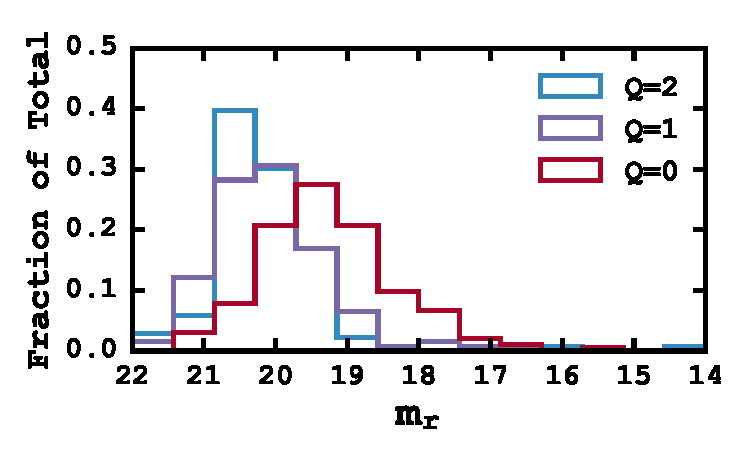
\includegraphics[width=0.6\textwidth]{figures2/redshiftHist.pdf}
	\end{center}
	\caption[Redshift recovery fractions across all clusters]{Redshift recovery fractions across all clusters. The bar heights represent the fraction of the total redshifts with the respective $Q$ value at a particular magnitude. For example, $\sim 40\%$ of the $Q=2$ redshifts have $m_r = 20.5-21$. We find a general decrease in redshift quality with increasing $m_r$. } 
	\label{2fig:redshiftHist} 
\end{figure}

Figure \ref{2fig:redshiftHist} shows the breakdown of $Q$ values for the redshifts across all clusters. We attempt to estimate spectroscopic redshifts for 447 galaxies, of which 44\% have $Q=0$, 27\% have $Q=1$ and 29\% have $Q=2$.  We find a general decrease in $Q$ flag with increasing $m_r$. Approximately 30\% of the $Q=0$ redshifts correspond to galaxies with $19 < m_r <20$ mag whereas about 40\% $Q=2$ galaxies have $m_r = 20.5-21$ mag.

\begin{landscape}
	\singlespace
	\begin{longtable}{ccccccccccc} 
	\caption[Spectroscopic redshifts for galaxies in VCSJ133520.1+410004.1]{Spectroscopic redshifts for galaxies in VCSJ133520.1+410004.1 measured with the MS: Column 1: The telescope pointing; Column 2: The dither position; Column 3: The fiber number; Column 4: The right ascension of the galaxy; Column 5: The declination of the galaxy; Column 6: The the observed SDSS \sdssr\ magnitude; Column 7: The galaxy redshift; Column 8: The redshift $Q$ flag; Column 9: The galaxy membership information; Column 10: The clustercentric radial distance; Column 11: The LOSV of the galaxy with respect to the cluster. See the appendix for similar tables for the remaining nine clusters.}\\
	\hline
	tile & dither & fiber & RA (J2000) & DEC (J2000) & \sdssr\ (mag) & redshift & $Q$ & Member & R (Mpc) & LOSV (\kms) \\
	(1) & (2) & (3) & (4) & (5) & (6) & (7) & (8) & (9) & (10) & (11) \\
	\hline \hline
	\endfirsthead
	\multicolumn{4}{l}%
	{\tablename\ \thetable\ Continued} \\
	\hline
	tile & dither & fiber & RA (J2000) & DEC (J2000) & \sdssr\ (mag) & redshift & $Q$ & Member & R (Mpc) & LOSV (\kms) \\
	(1) & (2) & (3) & (4) & (5) & (6) & (7) & (8) & (9) & (10) & (11) \\
	\hline \hline
	\endhead
		NE & 1 & 14 & 13:35:27.004 & +41:01:36.20 & 20.47 & 0.2019$\pm{0.0003}$ & 1 & ... & 0.40 & -6945$\pm{146}$ \\
		NE & 1 & 111 & 13:35:24.177 & +41:00:54.16 & 20.10 & 0.1178$\pm{0.0001}$ & 1 & ... & 0.15 & -27397$\pm{63}$ \\
		NE & 1 & 154 & 13:35:23.853 & +41:00:33.19 & 19.28 & 0.2214$\pm{0.0002}$ & 0 & ... & 0.18 & -2214$\pm{83}$ \\
		NE & 2 & 6 & 13:35:21.777 & +41:01:34.15 & 20.38 & 0.1691$\pm{0.0002}$ & 1 & ... & 0.27 & -14929$\pm{102}$ \\
		NE & 2 & 14 & 13:35:26.632 & +41:01:33.06 & 20.95 & 0.0403$\pm{0.0003}$ & 0 & ... & 0.09 & -46214$\pm{131}$ \\
		NE & 2 & 63 & 13:35:20.998 & +41:01:08.49 & 17.90 & 0.2381$\pm{0.0001}$ & 0 & $\checkmark$ & 0.25 & 1849$\pm{49}$ \\
		NE & 3 & 22 & 13:35:22.879 & +41:01:24.60 & 19.76 & 0.2386$\pm{0.0003}$ & 0 & $\checkmark$ & 0.33 & 1961$\pm{131}$ \\
		NE & 3 & 25 & 13:35:24.669 & +41:01:26.21 & 19.54 & 0.1444$\pm{0.0001}$ & 0 & ... & 0.25 & -20924$\pm{58}$ \\
		NE & 3 & 73 & 13:35:18.447 & +41:01:00.60 & 19.63 & 0.0779$\pm{0.0001}$ & 0 & ... & 0.09 & -37080$\pm{29}$ \\
		NE & 3 & 106 & 13:35:20.957 & +41:00:50.19 & 18.83 & 0.2235$\pm{0.0002}$ & 0 & $\checkmark$ & 0.17 & -1691$\pm{78}$ \\
		NE & 3 & 147 & 13:35:19.341 & +41:00:31.82 & 19.48 & 0.2380$\pm{0.0001}$ & 0 & ... & 0.11 & 1822$\pm{73}$ \\
		NE & 3 & 185 & 13:35:24.990 & +41:00:18.06 & 20.51 & 0.1887$\pm{0.0002}$ & 1 & ... & 0.18 & -10169$\pm{83}$ \\
		NE & 3 & 206 & 13:35:20.095 & +41:00:04.12 & 16.39 & 0.2274$\pm{0.0001}$ & 1 & $\checkmark$ & 0.00 & -763$\pm{34}$ \\
		NE & 3 & 210 & 13:35:22.528 & +41:00:05.00 & 19.59 & 0.2242$\pm{0.0001}$ & 1 & $\checkmark$ & 0.10 & -1543$\pm{49}$ \\
		NW & 1 & 127 & 13:35:16.384 & +41:00:47.33 & 17.43 & 0.2377$\pm{0.0001}$ & 0 & $\checkmark$ & 0.23 & 1752$\pm{68}$ \\
		NW & 1 & 167 & 13:35:14.400 & +41:00:29.73 & 19.69 & 0.2333$\pm{0.0002}$ & 0 & $\checkmark$ & 0.26 & 690$\pm{117}$ \\
		NW & 2 & 27 & 13:35:17.216 & +41:01:27.25 & 20.21 & 0.1512$\pm{0.0002}$ & 0 & ... & 0.24 & -19279$\pm{117}$ \\
		NW & 2 & 63 & 13:35:12.486 & +41:01:10.57 & 18.84 & 0.1638$\pm{0.0001}$ & 0 & ... & 0.31 & -16210$\pm{44}$ \\
		NW & 2 & 73 & 13:35:09.729 & +41:01:03.49 & 20.00 & 0.2402$\pm{0.0001}$ & 1 & ... & 0.50 & 2367$\pm{58}$ \\
		NW & 2 & 165 & 13:35:12.728 & +41:00:25.16 & 18.74 & 0.2394$\pm{0.0001}$ & 0 & $\checkmark$ & 0.33 & 2155$\pm{58}$ \\
		NW & 2 & 171 & 13:35:16.434 & +41:00:25.31 & 21.68 & 0.1617$\pm{0.0002}$ & 1 & ... & 0.13 & -16728$\pm{121}$ \\
		NW & 2 & 173 & 13:35:17.911 & +41:00:27.16 & 19.49 & 0.1039$\pm{0.0002}$ & 0 & ... & 0.06 & -30763$\pm{107}$ \\
		NW & 2 & 220 & 13:35:10.891 & +41:00:03.07 & 19.45 & 0.2994$\pm{0.0002}$ & 0 & ... & 0.47 & 16739$\pm{102}$ \\
		NW & 2 & 239 & 13:35:13.582 & +40:59:54.58 & 20.24 & 0.2316$\pm{0.0002}$ & 1 & $\checkmark$ & 0.28 & 265$\pm{92}$ \\
		NW & 3 & 142 & 13:35:16.981 & +41:00:35.55 & 19.44 & 0.2233$\pm{0.0002}$ & 0 & $\checkmark$ & 0.17 & -1745$\pm{78}$ \\
		SE & 1 & 27 & 13:35:25.896 & +40:59:52.05 & 19.35 & 0.2295$\pm{0.0004}$ & 1 & $\checkmark$ & 0.25 & -238$\pm{170}$ \\
		SE & 1 & 46 & 13:35:19.779 & +40:59:41.85 & 18.73 & 0.2293$\pm{0.0002}$ & 0 & $\checkmark$ & 0.08 & -284$\pm{107}$ \\
		SE & 1 & 86 & 13:35:26.506 & +40:59:28.30 & 20.59 & 0.2255$\pm{0.0002}$ & 1 & $\checkmark$ & 0.29 & -1205$\pm{112}$ \\
		SE & 1 & 123 & 13:35:22.588 & +40:59:11.02 & 18.17 & 0.2307$\pm{0.0002}$ & 0 & $\checkmark$ & 0.22 & 44$\pm{102}$ \\
		SE & 1 & 129 & 13:35:26.254 & +40:59:08.50 & 19.42 & 0.1282$\pm{0.0002}$ & 0 & ... & 0.20 & -24863$\pm{107}$ \\
		SE & 2 & 164 & 13:35:20.600 & +40:58:48.65 & 20.02 & 0.2938$\pm{0.0001}$ & 0 & ... & 0.33 & 15369$\pm{53}$ \\
		SE & 3 & 157 & 13:35:25.857 & +40:58:53.46 & 18.31 & 0.1701$\pm{0.0001}$ & 0 & ... & 0.28 & -14684$\pm{29}$ \\
		SE & 3 & 171 & 13:35:25.332 & +40:58:48.88 & 19.49 & 0.2400$\pm{0.0003}$ & 0 & ... & 0.36 & 2296$\pm{126}$ \\
		SE & 3 & 198 & 13:35:24.191 & +40:58:35.23 & 20.83 & 0.1177$\pm{0.0002}$ & 1 & ... & 0.21 & -27419$\pm{87}$ \\
		SW & 1 & 41 & 13:35:17.295 & +40:59:47.40 & 19.87 & 0.2231$\pm{0.0002}$ & 0 & ... & 0.13 & -1808$\pm{107}$ \\
		SW & 1 & 114 & 13:35:17.529 & +40:59:15.55 & 20.60 & 0.2493$\pm{0.0003}$ & 1 & ... & 0.22 & 4561$\pm{156}$ \\
		SW & 1 & 224 & 13:35:13.709 & +40:58:25.25 & 20.03 & 0.1276$\pm{0.0003}$ & 0 & ... & 0.28 & -25006$\pm{126}$ \\
		SW & 1 & 227 & 13:35:15.509 & +40:58:27.26 & 19.27 & 0.2328$\pm{0.0002}$ & 0 & $\checkmark$ & 0.41 & 559$\pm{83}$ \\
		SW & 1 & 245 & 13:35:17.832 & +40:58:19.02 & 19.29 & 0.2211$\pm{0.0003}$ & 1 & ... & 0.39 & -2275$\pm{136}$ \\
		SW & 1 & 246 & 13:35:18.529 & +40:58:20.43 & 21.31 & 0.1970$\pm{0.0002}$ & 1 & ... & 0.34 & -8140$\pm{117}$ \\
		SW & 2 & 24 & 13:35:15.282 & +40:59:51.52 & 21.29 & 0.2225$\pm{0.0002}$ & 1 & $\checkmark$ & 0.20 & -1934$\pm{97}$ \\
		SW & 2 & 29 & 13:35:18.391 & +40:59:50.06 & 18.17 & 0.2405$\pm{0.0001}$ & 0 & ... & 0.09 & 2440$\pm{44}$ \\
		SW & 2 & 39 & 13:35:15.539 & +40:59:43.86 & 18.73 & 0.2263$\pm{0.0002}$ & 0 & $\checkmark$ & 0.20 & -1023$\pm{107}$ \\
		SW & 2 & 53 & 13:35:15.211 & +40:59:38.90 & 18.73 & 0.2412$\pm{0.0001}$ & 0 & $\checkmark$ & 0.23 & 2593$\pm{58}$ \\
		SW & 2 & 59 & 13:35:09.857 & +40:59:32.82 & 19.83 & 0.2334$\pm{0.0002}$ & 1 & $\checkmark$ & 0.45 & 697$\pm{107}$ \\
		SW & 2 & 65 & 13:35:13.725 & +40:59:31.94 & 20.58 & 0.3156$\pm{0.0003}$ & 0 & ... & 0.37 & 20688$\pm{156}$ \\
		SW & 2 & 86 & 13:35:17.737 & +40:59:25.25 & 19.71 & 0.2236$\pm{0.0002}$ & 0 & $\checkmark$ & 0.17 & -1684$\pm{78}$ \\
		SW & 2 & 90 & 13:35:11.098 & +40:59:19.79 & 20.41 & 0.2354$\pm{0.0002}$ & 0 & $\checkmark$ & 0.42 & 1195$\pm{97}$ \\
		SW & 3 & 26 & 13:35:16.763 & +40:59:48.52 & 17.94 & 0.2250$\pm{0.0001}$ & 0 & $\checkmark$ & 0.15 & -1334$\pm{34}$ \\
		SW & 3 & 37 & 13:35:14.503 & +40:59:43.50 & 19.79 & 0.2428$\pm{0.0002}$ & 0 & $\checkmark$ & 0.26 & 2979$\pm{107}$ \\
		SW & 3 & 65 & 13:35:13.944 & +40:59:28.57 & 18.60 & 0.2362$\pm{0.0001}$ & 0 & $\checkmark$ & 0.29 & 1385$\pm{58}$ \\
		SW & 3 & 73 & 13:35:10.002 & +40:59:23.42 & 19.52 & 0.2307$\pm{0.0001}$ & 0 & $\checkmark$ & 0.45 & 39$\pm{73}$ \\
	\hline 
	\label{2tbl:VCSJ133520.1+410004.1} 
	\end{longtable}
\end{landscape}

\textsc{xcsao} reports errors on the cross-correlation redshift. Previous work \citeeg{Quintana2000, Sifon2015a} show the cross-correlation velocity uncertainties by up to a factor of two. We report our redshift uncertainties as twice the uncertainty estimated by \textsc{xcsao}.

Redshift information, with $Q=0$ or $Q=1$ spectra, for each galaxy are given in Table~\ref{2tbl:VCSJ133520.1+410004.1}. The right panel of Figure~\ref{2fig:VCSJ133520.1+410004.1} shows selected spectra from cluster VCSJ133520.1+410004.1 with corresponding best fitting SDSS template. See the appendix for similar examples from the remaining nine clusters.

\subsection{Cluster Membership}\label{2sec:cluster membership} 
We first determine the cluster central redshift. This serves as a zero-point from which all other galaxies will be compared. Therefore, the accurate determination of the cluster redshift ($z_c$) is crucial to the reliability of all following measurements. An incorrect cluster redshift introduces errors into the measured line of sight velocity (LOSV) and corresponding dispersion, which, in turn, contributes to errors associated with dynamical mass and radius. 

In simple terms, the cluster redshift is the mean of the redshifts of all galaxies associated with the cluster. However, because the standard mean can be quite sensitive to outliers or otherwise contaminated data, we require a more resistant statistic, and turn to the biweight location estimator \citep{Beers1990} which provides improved performance. The biweight location does not give us the freedom to use all galaxies measured but provides protection against a small number of interlopers. Therefore, the process of determining $z_c$ and the cluster membership are linked. We begin with the nominal $z_c$ (see Table~\ref{2tbl:targets}) and apply and initial velocity cut of 5000 \kms\ to remove any foreground or background galaxies. Then, using the membership determination techniques described below we determine the member galaxies from which a new $z_c$ is calculated. The entire process is repeated until convergence, usually within a single iteration. The cluster central redshift and associated 68\% uncertainties, derived from bootstrap resampling, are given in Table~\ref{2tbl: derived parameters}.

To reject the galaxies not associated with the targeted cluster, we employ two methods depending on the number of galaxies associated with each cluster. For clusters with 20 or more $Q=0$ or $Q=1$ redshifts we use the ``shifting gapper'' method of \citeeg{Fadda1996, Crawford2014}, which combines both the positional and velocity information. Galaxies are first sorted by their radial separation from the cluster center (See Table~\ref{2tbl:targets}) and binned into radial bins of at least 10 members. Once in the radial bins, the galaxies are sorted by the LOSV, 
\begin{equation}
	LOSV = c\frac{(z-z_{c})}{(1+z_{c})} 
\end{equation}
where $c$ is the speed of light in \kms, $z$ is the redshift of the individual galaxy and $z_{c}$ is the redshift of the cluster. Any galaxy with a LOSV greater than 1000 \kms of a neighboring galaxy (the velocity ``gap'') is rejected as an interloper. The procedure repeats until the number of galaxies stabilizes in the bin. Once the members have been identified we recompute $z_c$, LOSVs, and begin the membership selection again. This entire process is repeated until the number of member galaxies remains constant. This is normally achieved within a single iteration. 

For galaxy clusters with fewer than 20 $Q=0$ or $Q=1$ redshifts we employ the general of membership determination method outlined in \cite{Wilman2005, Connelly2012}. We assume an initial velocity dispersion, $\sigma(v)$, of 500$(1+z)$ \kms\ and apply both redshift and spatial limits given by: 
\begin{equation}
	\delta(z)_{max} = 2 \sigma(v)/c 
\end{equation}
and 
\begin{equation}
	\delta(r)_{max} = \frac{c\times\delta(z)_{max}}{bH(z)} 
\end{equation}
where $b=9.5$ is the aspect ratio between the projected spatial and line-of-sight dimensions, $H(z) = H_0 E(z)$ and $E(z) = \sqrt{\Omega_m(1+z^3)+\Omega_{\Lambda}}$. We select all galaxies with $|z-z_c| < \delta(z)_{max}$ and radial separation, $R$, $<\delta(r)_{max}$. During each step, we update both the $z_c$ and $\sigma(v)$ using the identified members and this process is repeated until the number of member galaxies converges, usually within three iterations.

To calculate the velocity dispersion in this membership determination method, we use the gapper estimator \citep{Beers1990} which provides accurate dispersions for groups as small as five members \citep{Hou2009}. It is given by 
\begin{equation}
	\sigma_g = \frac{\sqrt{\pi}}{N(N-1)} \sum_{i=1}^{N-1} w_i g_i
\end{equation}
where $N$ is the number galaxies, the weights are $w_i = i(N-i)$ and $g_i = LOSV_{i+1} - LOSV_i$ are the gaps between ordered pairs of radial LOSVs. The aspect  The dispersion estimate is corrected by $1.135$ to account for the $2\sigma$ redshift space cut applied during membership determination \citep{Connelly2012}. We follow this method for the calculation of the dispersion for consistency in member determination only. The final velocity dispersion of each cluster is determined in the following subsection.

Membership information for the galaxies observed in and around cluster VCSJ133520.1+410004.1 is given in Column 9 of Table~\ref{2tbl:VCSJ133520.1+410004.1}. See the appendix for the membership of the other observed clusters.

\subsection{Line-of-Sight Velocity Dispersion}\label{2sec:LOSVD}
To compute the line-of-sight velocity dispersion (LOSVD) of each cluster we follow the maximum likelihood method of \cite{Walker2006}. We assume that the each galaxy is drawn from a Gaussian distribution centered on the mean cluster velocity and we maximize the log of the product of each cluster member's individual Gaussian probabilities (their Eq. 8):
\begin{equation}
  \label{2eq:log}
\ln(p)=-\frac{1}{2}\sum_{i=1}^{N}\ln(\sigma_i^2+\sigma_p^2)-\frac{1}{2}\sum_{i=1}^N\frac{(v_i-\langle u \rangle)^2}{(\sigma_i^2+\sigma_p^2)}-\frac{N}{2}\ln(2\pi).
\end{equation}
where $N$ is the number of member galaxies, $\sigma_p$, $\langle\mu\rangle$, and $\sigma_i$ is the LOSVD, the average radial velocity and the error on the individual LOSVs respectively. To maximize the probability, we use {\sc emcee}\footnote{http://dan.iel.fm/emcee/current/} \citep{Foreman-Mackey2013}, a Monte Carlo Markov Chain (MCMC) sampler, based on affine-invariant ensemble sampler (see \citealt{Goodman2010} for details on affine-invariant samplers). We set priors on $\langle\mu\rangle$, and $\sigma_p$ by requiring that $\langle\mu\rangle$ lies between the maximum and minimum LOSV and that $\sigma_p$ be positive and less than $1400$ \kms which corresponds approximately to a $10^{16}$ \Msol\ cluster at $z=0$, larger than any expected cluster mass in our sample. We draw twenty thousand samples from the posterior probability distribution and report a measured LOSVD as the median value of the posterior probability distribution with 68\% error bars defined as the square root of the second moment of the same distribution.

\section{Estimating Cluster Masses}
The goal of this section is to describe the methods used to estimate (or predict) the total masses of the clusters in our sample. We test two distinct approaches. We begin the discussion with a traditional power law (PL) based approach where we estimate the cluster mass based on the LOSVD measurement. The second is a machine learning (ML) based approach where we use a combination of cluster observables to predict a cluster mass. The ML approach requires additional discussion about the creation of a suitable training set. We conclude with an examination of how this training set can potentially influence the results of the ML method.   

\subsection{PL Estimates of Cluster Mass}
We adopt the scaling relation of \cite{Munari2013} to estimate cluster masses based solely on their LOSVD. The scaling relation is based on the work of \cite{Evrard2008} and has the form: 
\begin{equation}\label{2eq:power law}
	M_{200c} = \frac{10^{15}}{h(z)} \bigg{(}\frac{\sigma_{1D}}{A_{1D}} \bigg{)}^{1/\alpha} \Msol 
\end{equation}
where $A_{1D} =1177\pm4.2$ \kms, $\alpha = 0.364\pm0.0021$, $h(z) = H(z)/100$, and $\sigma_{1D}$ is the LOSVD. The relation is calibrated through a cosmological simulation using galaxies (instead of dark matter particles or subhalos) as the tracers of LOSVD. This choice of tracer results in dynamical masses which are $16-26\%$ lower \citeeg{Kirk2015, Sifon2015a} than masses obtained through the scaling relation of \cite{Evrard2008}, which has been calibrated using dark matter particles alone. This is due dynamical effects which act upon the galaxies but not the dark matter particles.

We use the cluster redshift, given in Column 5, and the LOSVD values given in Column 6 of Table~\ref{2tbl: derived parameters} along with Equation~\ref{2eq:power law} to estimate the total mass of our ten clusters. The log of the estimated mass for each cluster is given in Column 7 of Table~\ref{2tbl: derived parameters}.

\subsection{Supervised Machine Learning}\label{2sec:ML methods}
Supervised ML provides an algorithm to infer the relationship between a set of known input variables (features) and a set of desired outputs (targets), through the use of a training set. The training set consists of both features and desired targets, which the ML algorithm uses to ``learn'' their relationship. The algorithm is then provided with a set of features alone, and uses the inferred relationship to predict appropriate target values. Part of the training set is often reserved as a \emph{testing} set \citeeg{Ripley2007, Xu2013, Ntampaka2015, Ntampaka2015a, Acquaviva2016} which is used to both select and train the specific ML algorithm.

Just as in \citetalias{Boada2016}, we rely on an ensemble ML method \citeeg{Caruana2006} known as a forest of randomized decision trees (or random forest; RF; \citealt{Ho1995, Ho1998}), which we prefer due to their straightforward design and easily accessible uncertainty estimates. A RF is a type of ensemble method where the trees can be visualized as flow chart. The path through the flow chart (the trees) is decided by the values of the training features at each fork. RF use a random subset of the train data to decide which fork should be followed. The final prediction is the mean of each tree's final value. We optimize the input parameters (often called hyper-parameters) of our RF by further splitting our testing set into a cross-validation (CV) set. We use 5-fold CV, where the testing set is split (folded) five times, throughout. The RF methods implemented in this work are part of the {\sc Scikit-Learn} \citep{Pedregosa2012} Python library.

Building off the work in \citetalias{Boada2016}, we use the ``Buzzard'' semi-analytical model to provide both the observable features and desired targets in order to train our ML method. The Buzzard mock galaxy catalog contains 238 million galaxies with \sdssr\ mag $< 29$ and $z \leq 8.7$. The galaxies are located in a 398.49 \degsq\ portion of the sky and their luminosities are derived from a combination of Sub-halo Abundance Matching (SHAM; \citealt{Reddick2013}) and Adding Density Dependent Spectral Energy Distributions (ADDSED). The galaxies are assigned to the dark matter halos identified by the {\sc ROCKSTAR} halo finder \citep{Behroozi2013}. The catalogs assume the following cosmological parameters: $\Omega_\Lambda = 0.714$, $\Omega_M = 0.286$, $\sigma_8 = 0.82$ and $H_0= 70$ \kms \mpc, which we have also adopted for general use in this work. See \citetalias{Boada2016} for a more thorough description of the process used to create the catalogs.

\subsection{ML Based Observations}

In order to create a mock dataset which resembles our actual observations we first rely on the RF method as a classifier. The goal is to assign each galaxy in the Buzzard catalog a $Q$ flag of either 0, 1 or 2 based on their observed magitudes in the five SDSS filters, \sdssu\sdssg\sdssr\sdssi\sdssz, the ten combinations of possible colors, and the square of those colors. \cite{Acquaviva2016} uses a similar feature set to predict the metallicity of SDSS galaxies with good effect. 

The classifier is trained using the redshift catalog derived from our cluster observations (Section \ref{2sec:redshift catalog}), and the 447 observations are split into a training, CV and test sample. We use the training set to train the ML method, the CV set to tune the model hyper-parameters and the test sample to verify how well our model classifies each galaxy. We also perform recursive feature elimination to remove features which contribute very little to the classification.

We compute two statistics to evaluate how well our model classifies the galaxies, the recall and the precision. The recall is the number predicted compared to the true number of classifications, $N_{pred}/N_{true}$. The precision is the number of correct predictions compared to the total number of predictions for each class, $N_{corr}/N_{pred}$. In both cases the metrics range from zero to one, and higher numbers are better. For our optimized RF classifier we achieve overall recall and precision of $\sim60\%$. For the individual classes ($Q$ flags), the RF classifier performs significantly better when classifying $Q=0$ and $Q=2$ galaxies, with recall rates well above 70\%. The $Q=1$ training galaxies have significant overlap between $Q=0$ and $Q=2$ (see Figure \ref{2fig:redshiftHist}) which leads to a recall for $Q=1$ galaxies of only $\sim20\%$. 

This is a difficult problem. Figure~\ref{2fig:redshiftHist} shows there is significant overlap between the $Q$ flags. In our testing, we find no combination of features which wholly separates the $Q$ flags, providing a high level of confusion for the RF. We find similar levels of recall and precision for other ML classification methods besides RF.

\begin{figure}[t]
	\begin{center}
		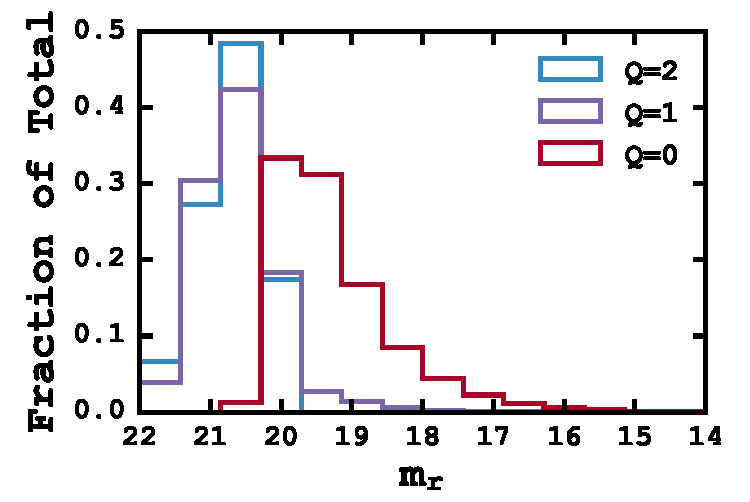
\includegraphics[width=0.6\textwidth]{figures2/buzzardQHist.pdf}
	\end{center}
	\caption[Quality flag assignments for the 2.7 million Buzzard catalog galaxies]{Quality flag ($Q$) assignments for the 2.7 million Buzzard catalog galaxies with $\sdssg< 22$ mag. The bar heights represent the fraction of the total redshifts with the respective $Q$ value at a particular magnitude. The distributions resemble the actual observations in Figure \ref{2fig:redshiftHist}. See the text for a detailed explanation of the classification process.} 
	\label{2fig:buzzardHist} 
\end{figure}

We assign each galaxy in the Buzzard catalog with $z<0.5$ and $\sdssg< 22$ mag a $Q$ flag using the optimized RF classifier trained with all 447 observations. Figure \ref{2fig:buzzardHist} shows the $Q$ flag distribution as a function of \sdssr\ magnitude. The total distribution of the 2.7 million $Q$ flags is 45.6\% $Q=0$, 24.7\% $Q=1$, and 29.6\% $Q=2$. This distribution closely resembles the fractions of the actual observations with some $Q=1$ galaxies misclassified as $Q=0$. Because we use galaxies with either $Q=0$ or $Q=1$ this is does not significantly bias our analysis.

\subsection{ML Based Cluster Masses}\label{2sec:ML based cluster masses}
We use the ``observed'' ($Q=0$ and $Q=1$) galaxies created in the previous subsection to construct total mass distributions of the mock clusters. For this task we again use a RF, not as a classifier but as a regressor, which predicts a cluster mass given a set of input features, such as the observed LOSVD and redshift. Similarly to our classification methods, we create an optimized ML method by splitting the Buzzard catalogs into a training, CV, and testing set. 

Because the cluster masses presented with this method are predictions based on the feature data, any uncertainties quoted by this method are prediction intervals not confidence intervals. Prediction intervals are an estimate of the interval encompassing future observations, with a given probability. Confidence intervals, on the other hand, describe the different moments of a population. The prediction intervals are unique to each prediction, and are often based on the underlying assumption of normally distributed residuals. RF estimators do not assume normally distributed residuals, and thus, require special treatment.  

The prediction intervals for our RF estimator as based on the method of quantile regression forests \citep{Meinshausen2006}. The basic principle is that we record all response variables (the predictions), not simply the mean. This allows us to give the prediction as the full conditional probability distribution of all possible predictions. For brevity, we quote predicted masses as the median prediction and the 68\% prediction interval as the square root of the second moment of the full conditional probability distribution.

\subsection{The Importance of Training Features}\label{2sec: training features}
\begin{figure}[t]
	\begin{center}
		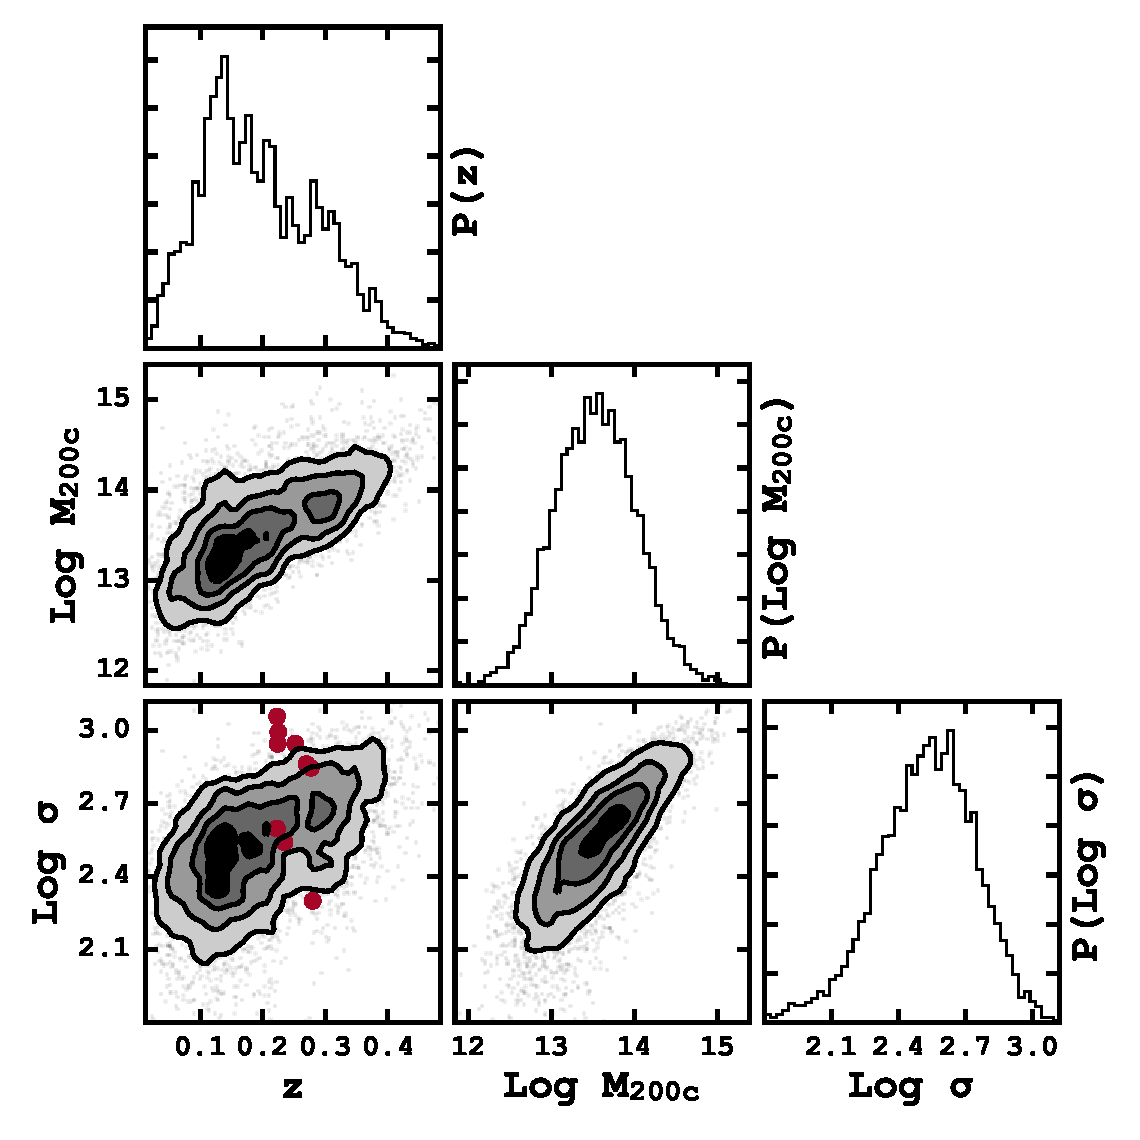
\includegraphics[width=0.6\textwidth]{figures2/buzzardCorner.pdf}
	\end{center}
	\caption[Corner plot of the \emph{training} data with features $\sigma$ and $z$.]{Contour plot of the \emph{training} data with features $\sigma$ and $z$. The corner plots shows all of the one and two dimensional posterior probability distributions used to determine the correct cluster mass. The colored circles show the position in the log $\sigma$-redshift plane of the ten clusters in this sample.}
	\label{2fig:buzzardCorner}
\end{figure}

The data used to train our ML algorithm is critical to the success of the method. We require training data which is broad enough to expose the ML method to a wide enough range of cluster parameters as not to influence the final outcome. The features of our training sample can be selected such that it does not bias the final predictions in an expected way. Figure~\ref{2fig:buzzardCorner} shows the $\sigma$ and $z$ features of the training sample from the Buzzard catalogs.\footnote{Contour plots based on \cite{Foreman-Mackey2016}.} The large red circles indicate the observed positions of our ten clusters in relation to the training data. Immediately noticeable, is that our observed clusters occupy a narrow redshift range ($0.2< z <0.3$). We also notice that seven of the ten clusters sit at the top edge of the training data in the $z$-log $\sigma$ plane. Because the observed clusters are separate from the training data, the accuracy of the predictions of the cluster masses will be diminished. 

Because the of the difference in cosmological volume covered by the SDSS and simulated by Buzzard, there are too few clusters in Buzzard, at $z\sim2$, and with $\sigma$ as large as the clusters in our sample. Predictions based on the Buzzard catalogs give a higher likelihood that clusters at $z\sim2$ will be of lower total mass, when the redshift is included as a feature. This becomes apparent by examining the $z$-log $M_{200c}$ plane in Figure~\ref{2fig:buzzardCorner}. The vast majority of clusters with $0.2< z <0.3$ have masses between $10^{13} - 10^{14}$ \Msol, whereas the observed LOSVD ($\sigma$) values of our clusters would place them above $10^{15}$ \Msol. 

To combat the effect of cluster mass under-prediction, we make two critical changes from our method presented in \citetalias{Boada2016}. First, instead of using the membership information provided by the Buzzard catalogs we observe the clusters much in the same way we have with our actual observations. We select all galaxies within $2\farcm3$ around the center of each cluster (see Figure~\ref{2fig:tiles} for an illustration), and determine the cluster membership using the methods described in Section~\ref{2sec:cluster membership}. This serves to broaden the LOSVD distribution of the training data as both true member galaxies will be excluded and interloping galaxies will be erroneously included. Secondly, we exclude the redshift information from the training features when predicting the cluster masses. This has the effect of flattening the HMF, allowing for high mass clusters to exist at all redshifts. However, the fewer training features also lowers the predictive power through an increase in both the bias and scatter (see Figure 6 in \citetalias{Boada2016} as an example). 

\section{Results and Discussion}\label{2sec:results}
The goal of this work to perform a practical test of some of the potential applications of a HETDEX-like survey to cluster science. Here, we present the predicted total masses of our ten clusters and estimate the absolute scale and scatter of a richness-mass relation based on those cluster masses. Because the accuracy of the predicted cluster masses is paramount to a well constrained richness-mass relation, we combine our results presentation with a discussion on their accuracy. 
 
\subsection{Cluster Masses}
\begin{figure} 
	% \includegraphics[width=\columnwidth]{figures/MLcomparison_shifty.pdf}
	\begin{center}
		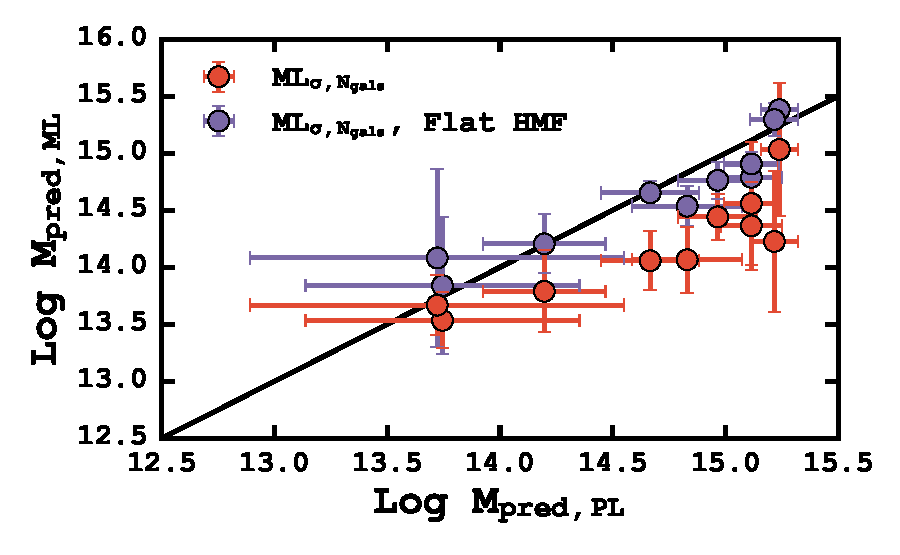
\includegraphics[width=0.6\textwidth]{figures2/massCompare.pdf} 
	\end{center}
	\caption[PL estimated cluster versus ML predicted cluster mass]{Comparison of the cluster mass estimates for the PL scaling relation (Equation~\ref{2eq:power law}) and the ML based mass predictions. We find the ML method sigificantly underestimates the cluster mass when compared to the PL method. This is due to the ML's reliance on training data which does not wholly represent the our sample of observed clusters.}
 \label{2fig: ML comparison} 
\end{figure}

In \citetalias{Boada2016} we find the ML based method with the LOSVD ($\sigma$), redshift ($z$) and number of galaxies observed ($N_{gal}$) showed both the smallest bias and scatter over the largest range of cluster masses. This worked well because the training data were selected from a volume of similar size to the survey in question. As discussed previously, we modify our analysis slightly and use the PL based approach (Eqn.~\ref{2eq:power law}) and the $\mathrm{ML}_{\sigma, N_{gal}}$ method to estimate the masses of our ten clusters. This change in the ML method is the result of the differences in the cosmological volume of the SDSS and the Buzzard at $z\sim2$.  

The PL predicted masses versus the ML predicted masses are shown in Figure~\ref{2fig: ML comparison}. We find that the PL based mass estimates are significantly higher than the ML based predictions, due to the ML relying on the biased training set discussed previously. In \citetalias{Boada2016}, the cluster mass prediction process uses two steps. Firstly the cluster mass is predicted, and then the cluster mass is corrected by considering the bias and scatter of the training data. Here, we choose to not correct the cluster masses predicted by either method due to the dissimilarity between the training data and our observations. During our testing, we find that there are too few training clusters with masses $> 10^{15}$ \Msol\ to place reliable contraints on the bias and scatter. As we discuss below, these high mass cluster constitute the bulk of our sample. Because we are unable to provide these clusters, with bias corrections, we choose to not correct any cluster mass estimate, to facilitate consistency throughout. 

The lack of a bias correction does not strongly effect our analysis as we are primarily interested in the scatter of our cluster masses. The scatter is unaffected as the individual mass estimates are scaled up or down by a common factor.

% The prediction process uses two steps. Firstly, we use a method to predict the individual masses and secondly we correct those masses based on the results of the training data. The upper panel of Figure~\ref{2fig: ML comparison} shows the cluster mass predictions for the Buzzard catalog clusters using the PL and $\mathrm{ML}_{\sigma, N_{gal}}$ approaches. The black diagonal line shows the 1:1 relation. The lower panel of Figure~\ref{2fig: ML comparison} shows the fractional error
% \begin{equation}\label{2eq: fractional error}
% 	\epsilon = (M_{pred} - M_{200c})/M_{200c}
% \end{equation}
% as a function of true cluster mass, $M_{200c}$ from the simulation.
%
% Using the predicted cluster masses for the Buzzard catalog we can quantify the amount of bias, and the scatter about that bias for different bins of predicted cluster mass. The bias is correctable by simply shifting our predicted cluster mass up or down by the appropriate amount. The scatter estimates the overall mass scale uncertainty in each bin of predicted cluster mass. We report the uncertainties in our cluster mass estimates as the sum in quadrature of the either confidence interval of the PL method or the prediction interval from the ML method and the mass scale uncertainty discussed here.

\begin{landscape}
	\begin{table}
	\caption[Summary of derived cluster parameters.]{Summary of derived cluster parameters: Column 1: The cluster name; Column 2: The number of SDSS sources observed; Column 3: The number of $Q=0(1)$ sources; Column 4: The number of member galaxies; Column 5: The redshift of the cluster; Columns 6: The LOSVD; Column 7: The PL predicted cluster mass; Column 8: The ML predicted cluster mass.} 
	\begin{tabular}{lccccccc} 
		\hline 
		&&&&&& PL & ML \\
		Cluster & Sources & Q=0 (1) & Member & $z_{c}$ & $\sigma$ (\kms) & log $M_{pred}$ & log $M_{pred}$ \\
		(1) & (2) & (3) & (4) & (5) & (6) & (7) & (8) \\
		\hline \hline 
		VCSJ010455.4+000336.3 & 41 & 10 (10) & 15 & 0.2727$\pm{0.0029}$ & 1194$\pm{135}$ & 15.11$\pm{0.14}$ & 14.84$\pm{0.18}$ \\
		VCSJ133520.1+410004.1 & 67 & 35 (17) & 25 & 0.2310$\pm{0.0025}$ & 1314$\pm{91}$ & 15.24$\pm{0.08}$ & 14.71$\pm{0.47}$ \\
		VCSJ140102.0+025242.6 & 67 & 14 (30) & 16 & 0.2543$\pm{0.0035}$ & 1295$\pm{115}$ & 15.22$\pm{0.11}$ & 14.55$\pm{0.45}$ \\
		VCSJ153656.3+242431.6 & 37 & 14 (14) & 11 & 0.2255$\pm{0.0034}$ & 932$\pm{189}$ & 14.83$\pm{0.24}$ & 14.21$\pm{0.16}$ \\
		VCSJ164019.8+464241.5 & 61 & 36 (14) & 32 & 0.2274$\pm{0.0020}$ & 1183$\pm{121}$ & 15.11$\pm{0.12}$ & 14.96$\pm{0.23}$ \\
		VCSJ172227.2+320757.2 & 61 & 26 (18) & 23 & 0.2260$\pm{0.0022}$ & 1044$\pm{154}$ & 14.97$\pm{0.18}$ & 14.54$\pm{0.14}$ \\
		VCSJ211849.1+003337.3 & 45 & 21 (8) & 18 & 0.2750$\pm{0.0026}$ & 820$\pm{148}$ & 14.67$\pm{0.22}$ & 14.30$\pm{0.12}$ \\
		VCSJ215422.9+003723.5 & 28 & 19 (2) & 16 & 0.2167$\pm{0.0026}$ & 547$\pm{124}$ & 14.20$\pm{0.27}$ & 14.04$\pm{0.09}$ \\
		XMMXCSJ124425.9+164758.0 & 25 & 11 (8) & 6 & 0.2316$\pm{0.0033}$ & 375$\pm{191}$ & 13.75$\pm{0.61}$ & 13.60$\pm{0.14}$ \\
		XMMXCSJ125650.2+254803.2 & 15 & 8 (3) & 3 & 0.2821$\pm{0.0059}$ & 372$\pm{258}$ & 13.72$\pm{0.83}$ & 13.52$\pm{0.13}$ \\
		\hline 
		\end{tabular}
		\label{2tbl: derived parameters} 
	\end{table}
\end{landscape}

Table~\ref{2tbl: derived parameters} presents a summary of the derived parameters for each cluster. We include the LOSVD, the estimated cluster redshift, and the number of member galaxies observed. We provide two predicted cluster masses, the PL based cluster mass and the $ML_{\sigma, N_{gal}}$ predicted cluster mass. We discuss the accuracy of both of these predictions in the following subsections.

\subsection{Notes for Individual Clusters}
Here we compare our PL inferred masses for the clusters in our sample to the previously reported estimates from the literature. \cite{Sifon2015} report total cluster masses for four of our clusters based on LOSVD measured from targeted spectra obtained with the Canada-France-Hawaii Telescope. They convert the LOSVD into a dynamical cluster mass using the PL scaling relation of \cite{Evrard2008} (which is the basis of our Equation~\ref{2eq:power law}) and estimate the uncertainties using jackknife resampling. One of our clusters has a reported LOSVD measurement and two have X-ray temperature measurements. In the following section we will discuss the ML estimated masses.

\subsubsection{VCSJ133520.1+410004.1 (Abell 1763)}
\cite{Sifon2015} observe 103 member galaxies within $r_{200}$. The compute a LOSVD of 1130$\pm81$ \kms, compared to our 1314$\pm91$ \kms\ based on 25 member galaxies. They report a $M_{200c} = (14.6\pm3.1) \times 10^14$ \Msol, compared to our value of $M_{200c} = (17.4\pm3.2) \times 10^14$ \Msol. The two estimates are consistent within the given errors, and the difference is due to our higher measured LOSVD.

\subsubsection{VCSJ140102.0+025242.6 (Abell 1835)}
\cite{Sifon2015} report a $M_{200c} = (4.5\pm1.9) \times 10^14$ \Msol, based on 41 member galaxies within
$r_{200c}$. We estimate a significantly different mass of $M_{200c} = (16.6\pm4.2)\times 10^{14}$ \Msol.
This discrepancy is due to the large difference in measured LOSVD, 762$\pm106$ \kms\ versus our
1295$\pm115$ \kms. However, \cite{Hoekstra2012} report a LOSVD for VCSJ140102.0+025242.6 of 1218 \kms.
\cite{Geller2013} find $M_{200c} = (16.57\pm1.86)\times 10^{14}$ \Msol\ from the best fitting caustic mass
profiles, which is similar to our reported value. Using \emph{Chandra} X-ray observations,
\cite{Bonamente2012} report a $M_{200c} = (8.35$\err{0.86}{0.81}$)\times 10^{14}$ \Msol. While our cluster
mass estimate is not consistent with \cite{Sifon2015}, we find it is very similar to other reported mass
estimates based on virial techniques.

\subsubsection{VCSJ164019.8+464241.5 (Abell 2219)}
With the largest number of member galaxies observed (of our sample), \cite{Sifon2015} use 241 member galaxies within $r_{200c}$ to estimate a mass of $M_{200c} = (17.0\pm2.8)\times 10^{14}$ \Msol. We estimate $M_{200c} = (12.9\pm3.6)\times 10^{14}$ \Msol. Using weak lensing techniques, \cite{Applegate2014} report a mass of $(12.0$\err{1.5}{1.5}$)\times 10^{14}$ \Msol\ within 1.5 Mpc, similar to our reported mass estimate.

\subsubsection{VCSJ172227.2+320757.2 (Abell 2261)}
For VCSJ172227.2+320757.2 we estimate $M_{200c} = (9.3\pm3.9)\times 10^{14}$ \Msol\ compared to $M_{200c} = (7.0\pm2.0)\times 10^{14}$ \Msol from \cite{Sifon2015}. They base their estimate on 76 member galaxies within $r_{200c}$. There is reasonable agreement between the two estimates.

\subsubsection{VCSJ215422.9+003723.5 (Abell 2392)}
The predicted mass of this cluster is significantly lower than expected. Previous work \citep{Wing2013} find it has a LOSVD of 1485 \kms\ well outside the estimated value from our analysis of $547\pm124$. \cite{Wing2013} report a LOSVD based on 32 member galaxies within 3 Mpc of the cluster center. One possible explanation for the deviation between our result and that of \cite{Wing2013} is that our observations probe only the cluster core ($<0.4$ Mpc), while their measurements include galaxies much farther away. Previous theoretical work \citeeg{Old2013} has shown the LOSVD to be sensitive to the radius at which it is measured. In addition, there is evidence to suggest that the cores of some galaxy clusters exhibit a smaller velocity dispersion than the outskirts \citeeg{Bahcall1977, Muriel2002}.

\subsubsection{XMMXCSJ124425.9+164758.0}
With only six member galaxies identified, XMMXCSJ124425.9+164758.0 is near the very limit of our ability to produce accurate cluster mass estimates. Fortunately, the cluster has an measured x-ray temperature which we can use to as another estimate of mass. Its XCS data release 1\footnote{http://www.astro.ljmu.ac.uk/$\sim$xcs/DR1/XCSDataRelease.html} \citep{Mehrtens2012} measured temperature is 1.3\err{0.3}{0.2} KeV which equates to $M_{500c}\approx(0.41\pm0.08)\times10^{14}$ \Msol\ using the $T_x$-M relationship for low-temperature systems of \cite{Finoguenov2001}.

We convert this X-ray inferred mass from $M_{500c}$ to $M_{200c}$ using the general prescription in \cite{Hu2003} to arrive at a predicted mass of $M_{200c} \approx (0.53\pm0.11)\times10^{14}$ \Msol, in very good agreement with our LOSVD predicted value of $M_{200c} \approx (0.59\pm0.81)\times10^{14}$ \Msol.

\subsubsection{XMMXCSJ125650.2+254803.2}
The three member galaxies identified in XMMXCSJ125650.2+254803.2 do not place a statistically strong constraint on the LOSVD predicted cluster mass. It too has a X-ray temperature measurement as part of XCS. Using the same approach as with XMMXCSJ124425.9+164758.0, a measured X-ray temperature of 1.4\err{0.3}{0.2} KeV gives a X-ray inferred cluster mass of $M_{200c} \approx 0.61\times10^{14}$ \Msol. This is about 26\% higher than our LOSVD derived cluster masses. 

\subsection{On the Accuracy of ML based Cluster masses}
Many of the cluster masses predicted using the ML approach are significantly different from both the PL based masses and the values found in the literature. Specifically, the largest differences are for the high mass clusters, and this can wholly be attributed to the training data used to inform the ML method (see the discussion in Subsection~\ref{2sec: training features}). 

In \citetalias{Boada2016} we found significantly reduced scatter in our mass predictions through the use of ML methods. We argue that the amount of scatter and cluster mass accuracy are reasonable estimates of those for a survey such as HETDEX. In large part, this is because the cosmic volume probed by HETDEX is of similar size to that simulated by Buzzard. However, the clusters observed for this work are selected from the SDSS which covers a much larger cosmological volume. The smaller simulated volume of Buzzard leads to the issue where the training data does not accurately represent the population of clusters in question.

Simply, Buzzard lacks the intermediate redshift, high-mass cluster, which influences the ML predictions of the cluster mass. Improvements in the accuracy of the ML method are possible by (re-)introducing the cluster redshift as a feature (see \citetalias{Boada2016} as an example), but that would require a training dataset that has the same area/depth as the dataset used for the observations, in this case, the SDSS.

The prediction intervals output by the ML method also show the effect of the mis-matched training sample. The ML prediction intervals are narrower than the PL-inferred confidence intervals for all clusters with masses below $10^{15}$ \Msol. This is due to an abundance of training clusters in this range. Above this, there are too few clusters to give reliable predictions and the prediction interval widens to reflect that situation.

It is important to note, that the cluster mass predictions from the ML methods are not a failure of the method. Based on the training data the algorithm has been exposed to, it has predicted cluster masses which closely resemble the observed features. Supervised ML shows incredible promise as a tool for future astrophysical investigations, but a deep understanding of how the input training data effects the target output is also required.

\subsection{Optical Richness-Mass Relation}
\begin{figure}
	\begin{center}
		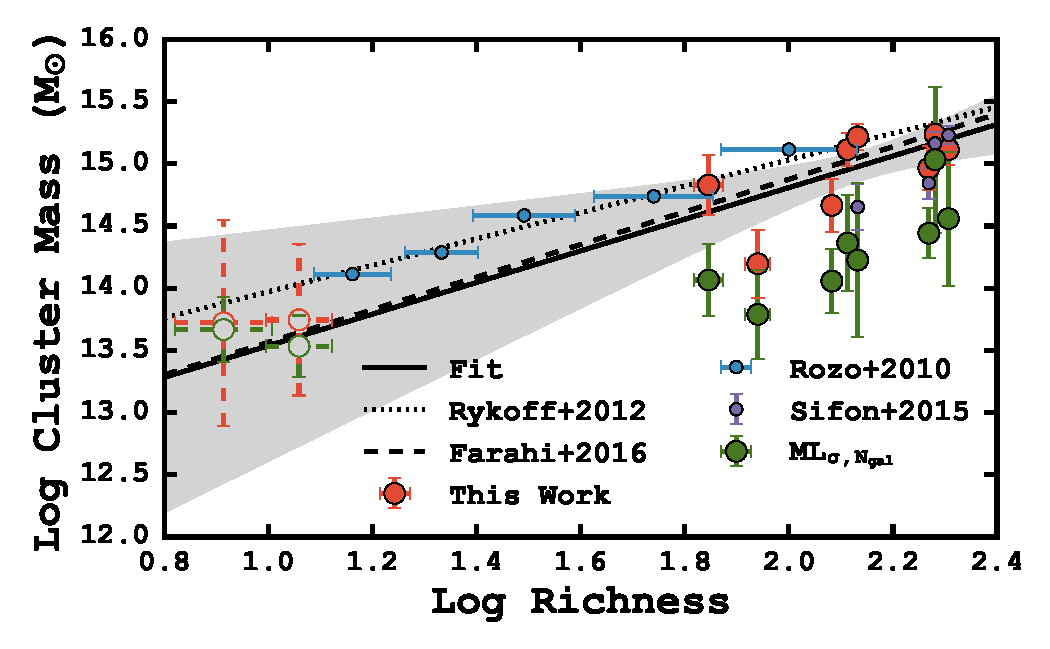
\includegraphics[width=\textwidth]{./figures2/massRichness.pdf} 
	\end{center}
	\caption[Richness versus total cluster mass for the clusters in our sample]{Richness, $\lambda$, versus total cluster mass for the clusters in our sample, shown as orange points. The two dashed points are the X-ray selected clusters, and are excluded from the fit. The solid black like shows our best-fitting relation (Equation~\protect\ref{2eq: best fit}) based on the eight high mass clusters, the dashed line shows the relation from \protect\cite{Farahi2016}, and the dotted line shows the relation from \protect\cite{Rykoff2012}. The gray shaded region corresponds to the 68\% confidence area on our best-fit. We also include stacked WL masses from \protect\cite{Rozo2010} and the high-mass cluster mass estimates of \protect\cite{Sifon2015} for comparison.}
\label{2fig:massRichness} 
\end{figure}

In \citetalias{Boada2016}, we show that HETDEX will be able to accurately estimate the absolute calibration and intrinsic scatter, $\sigma_{M|\lambda}$, of the optical-richness-cluster-mass relationship for a small range of intrinsic scatters. Here we use the ten clusters observed to demonstrate the ability of IFU observations similar to HETDEX to make mass determinations and to use those masses to place constraints on the optical-richness-cluster-mass relation. For our cluster mass estimates we use the masses predicted by the PL relation given in Equation~\ref{2eq:power law}. 

To find a best-fitting richness-mass relation for our data we are required to fit $y=mx+b$ where $y =$ log predicted cluster mass and $x =$ log optical richness, considering measurement errors in richness and predicted cluster mass along with intrinsic scatter of the relation. We assume the intrinsic scatter is constant from point to point, and we assume (not necessarily correctly) that all measurement errors are Gaussian. With the assumption of all Gaussian scatters we have three quantities of interest:
The probability of the predicted log cluster mass ($y_i$) given the observed log richness ($x_i$),
\begin{equation}\label{2eqn:intrinsic scatter}
	p(y_i|x_i) = \frac{1}{\sqrt{2\,\pi\,\sigma^2}}
	 \,\exp\left(-\frac{[y_i - m\,x_i - b]^2}{2\,\sigma^2}\right)
\end{equation}
which takes into consideration the intrinsic scatter in the relation, $\sigma$; the probability of the true log richness value ($\hat{x_i}$) given an observed log richness ($x_i$),
\begin{equation}\label{2eqn:xerr}
	p(\hat{x_i}|x_i) = \frac{1}{\sqrt{2\,\pi\,\sigma_{x,i}^2}}
	 \,\exp\left(-\frac{[\hat{x_i} - x_i]^2}{2\,\sigma_{x,i}^2}\right)
\end{equation}
which accounts for the uncertainty in the richness observation, $\sigma_{x,i}$; and the probability of the true log cluster mass ($\hat{y_i}$) given an observed log cluster mass ($y_i$),
\begin{equation}\label{2eqn:yerr}
	p(\hat{y_i}|y_i) = \frac{1}{\sqrt{2\,\pi\,\sigma_{y,i}^2}}
	 \,\exp\left(-\frac{[\hat{y_i} -y_i]^2}{2\,\sigma_{y,i}^2}\right)
\end{equation}
which also considers the uncertainty associated with the log cluster mass prediction, $\sigma_{y,i}$. We combine these three probabilities into
\begin{equation}
	p(\hat{y_i}|\hat{x_i}) = \int_{-\infty}^\infty dy_ip(\hat{y_i}|y_i) \int_{-\infty}^\infty dx_ip(y_i|x_i)p(x_i|\hat{x_i}).
\end{equation}
We assume flat priors on $x_i$ so that $p(x_i|\hat{x_i}) = p(\hat{x_i}|x_i)$ and substitute our probability equations from above. This gives
\begin{equation}
	p(\hat{y_i}|\hat{x_i}) = 
	\frac{1}{\sqrt{2\,\pi\,(\sigma^2 + \sigma_{y,i}^2 + m^2\sigma_{x,i}^2)}}\exp\left(-\frac{[y_i - m\,x_i - b]^2}{2\,(\sigma^2 + \sigma_{y,i}^2 + m^2\sigma_{x,i}^2)}\right)
\end{equation}
which for $\sigma_{x,i}=0$ (no uncertainty on the log richness measurement) reduces to the familiar form of a Gaussian with a combination of measurement error and intrinsic scatter. We convert this probability function into a likelihood by taking the product of all the individual probabilities,  
\begin{equation}\label{2eq:like}
\mathscr{L} = \prod_{i=1}^N \ p(\hat{y_i}|\hat{x_i}).
\end{equation}
and maximize this likelihood by sampling from the posterior probability distribution using the MCMC methods described above. We quote the most probable slope and intercept as the mean value of the posterior probability distributions with uncertainties as the square root of the second moment of the same distribution.

To find our best-fitting relation we exclude the two \emph{XMM} selected clusters due to the few number of observed member galaxies. After fitting to the remaining eight, high richness clusters, we find a best-fitting relation of 
\begin{equation}\label{2eq: best fit}
 \mathrm{Log}\,M_{200c}=1.25\pm{0.78}\, \mathrm{Log}\,\lambda + 12.29\pm{1.68}. 
\end{equation}
This best-fitting relation is shown in Figure~\ref{2fig:massRichness} where the large filled, orange points are the PL estimated cluster masses from this work, and the dashed points are the excluded \emph{XMM} selected clusters. We comment on the properties of our optical richness-mass relation and compare it to others from the literature in the following subsection.

We estimate the intrinsic scatter, $\sigma_{M|\lambda}$, in the relation two ways. The first is through our generative model, as it includes an intrinsic scatter term, which the MCMC samples directly. This gives $\sigma_{M|\lambda} = 0.23\pm0.16$ dex for the intrinsic scatter. We can also calculate the standard deviation of the residuals to the best-fitting line, which produces $\sigma_{M|\lambda} = 0.27\pm0.07$ dex. Both of these scatter estimates include the eight $\lambda > 60$ clusters. If we exclude VCSJ215422.9+003723.5 where we significantly underestimate the mass, the scatter for remaining seven clusters is $\sigma_{M|\lambda} = 0.24\pm0.09$ dex.

\subsection{Calibration of the Richness-Mass Relation}
We begin with a brief discussion of our best-fitting richness-mass relation. Two recent studies \citep{Farahi2016, Simet2016} use stacked cluster observations of velocity dispersions or WL, and it both cases report a PL index of $\alpha\sim1.33$. We find a similar (6\% difference) PL index of $\alpha\sim1.25$, albeit with significant uncertainty. Our absolute mass scale of log $M_{200c}/\Msol = 14.29\pm2.1$ dex at $\lambda=40$ is in good agreement with the previously reported values of log $M_{200c}/\Msol \sim 14.29$ dex, although with much greater uncertainty. These large uncertainties are due to our sample having so few reliable cluster mass estimates; our fitting procedure cannot place tight constraints on the measured slope and intercept. With the many clusters expected to be observed with HETDEX these uncertainties should decrease significantly.

% We begin with a brief discussion of the richness-mass relation itself. Because we have selected our clusters from the redMaPPer catalog, we begin with the richness-mass relation from \cite{Rykoff2012}. The authors suggest a PL index of $\alpha=1.06$ and an absolute mass scale of Log $M_{200c}/\Msol=14.64$ at $\lambda=60$. We find a 16\% difference in the slope, and a lower absolute mass scale of Log $M_{200c}/\Msol = 14.57\pm1.07$. \cite{Rykoff2012} go on to note that their relationship is not rigorously measured, so this discrepancy is unsurprising.

The individually measures cluster masses allow us to place promising constraints on the scatter in cluster mass at fixed richness, $\sigma_{M|\lambda}$. Using the SZE, \cite{Saro2015} find $\sigma_{M|\lambda} \sim 0.18$ at $\lambda = 70$. \cite{Rykoff2016} identify a similar scatter of $0.3\pm0.15$ using X-ray scaling relations and the DES science verification dataset. Many other studies \citeeg{Baxter2016, Farahi2016, Simet2016} adopt a $\sigma_{M|\lambda}\sim 0.2-0.3$ dex \citep{Rozo2014, Rozo2015}. These values correspond well to our value of $\sigma_{M|\lambda} = 0.24\pm0.09$ dex, and the $0.2-0.3$ range corresponds well to the region most sensitively probed in our simulated HETDEX survey \citepalias{Boada2016}.

The ability of blind spectroscopy to constrain both the absolute cluster mass scale and, more importantly, the amount of scatter at fixed optical richness to values similar to other techniques is extremely positive for the potential of HETDEX. As cluster mass estimates become better constrained through the use of ML methods, we can expect to find even tighter constrains on the optical richness-cluster mass relation. This should lead to excellent calibration of other large-area sky surveys which produce optical photometry only. In addition, it will serve as an important, independent check on other observable-cluster mass relationships which are often noisy and subjet to large systematic uncertainties \citeeg{Sereno2015}.

\section{Summary}\label{2sec:summary}
We carry out a proof-of-concept study where we present integral field unit observations with the Mitchelle Spectrograph of ten intermediate redshift ($z=0.2-0.3$) galaxy clusters. We observe cluster member galaxies within $R\sim0.5$ Mpc of each cluster, and determine each cluster's membership based on the line-of-sight velocity of each galaxy. The mass of each cluster is determined through a traditional PL and through a machine learning based approach. We use these estimates of cluster mass to measure the absolute mass scale and intrinsic scatter of the optical richness-cluster mass relationship. The goal of this study is to investigate how a blind spectroscopic survey, such as the forthcoming Hobby Eberly Dark Energy Experiment (HETDEX), will be able to predict cluster masses, and then to use those masses to help calibrate other observable-cluster mass scaling relations.
Our main results are as follows:
\begin{itemize}
	\item Using a PL scaling relation between the measured line-of-sight velocity dispersion and cluster mass, our low richness ($\lambda < 15$) sample of galaxy clusters have total inferred masses $\sim 0.5 \times 10^{14}$ \Msol\ ($M_{200c}$), and the high richness ($\lambda > 60$) cluster sample has total masses $(1.58-17.37) \times 10^{14}$ \Msol\ ($M_{200c}$). The majority of these estimate are consistent with other published total mass estimates which use a variety of estimation techniques. 
	
	\item The machine learning based approach of galaxy cluster mass estimation, while powerful, requires a deep understanding of both the machine learning algorithms available, and expert knowledge of the problem domain. To estimate the total masses of the galaxy clusters in our sample using machine learning methods, the Buzzard catalogs do not provide a suitable training set due to the limited cosmological volume simulated at low redshift. For the redshift range of our cluster sample, the Buzzard catalogs lack similar high velocity dispersion clusters. This leads to a severe down-weighting of high mass galaxy clusters when the cluster redshift is included as a training feature. When this feature is removed, the machine learning estimated cluster masses improve but are still underestimated due to too few very high mass clusters being included in the simulated volume. A suit a training data drawn from a similarly sized cosmological volume is critical to the reliable prediction of cluster masses. When this is available, the machine learning predicted cluster masses show less bias and lower scatter compared to a traditional power law scaling relation based on velocity dispersion alone.

	\item We fit a optical richness-cluster mass relation to the eight high richness ($\lambda > 60$) clusters. This gives:
		\begin{equation}
			\mathrm{Log}\,M_{200c}=1.25\pm{0.78}\, \mathrm{Log}\,\lambda + 12.29\pm{1.68}.  
		\end{equation}
We are unable to place tight constraints on the overall estimate of the normalization due to the relatively few clusters included. We do estimate the scatter in cluster mass at fixed richness, $\sigma_{M|\lambda} \sim 0.25$. This estimate of scatter compares well with other recent studies of the richness-mass relation. This suggests that a blind spectroscopic survey such as HETDEX will be able to provide a crucial, independent measurement of this scatter, to a much high precision than is possible in this work. This bodes well for the success of HETDEX as not only a high redshift galaxy survey but as a important calibration tool for understanding the uncertainties associated with galaxy cluster mass estimates. 
\end{itemize}
